% SENG3011 Testing Documentation
\title{Testing Report}
\author{Nicholas Grasevski \and Daniel Morton \and George El-Boustani \and Christopher Tin-Loi}
\date{\today}

\documentclass{article}
\usepackage{graphicx}

\begin{document}
\maketitle

% Teams must produce 1 document describing the testing processes used in the
% development of the product and attach their testing data.

\section{Architecture}
% The latest version of your architecture. Indicate which components are
% being tested and the type of testing (functional or non-functional)

\begin{figure}
\centering
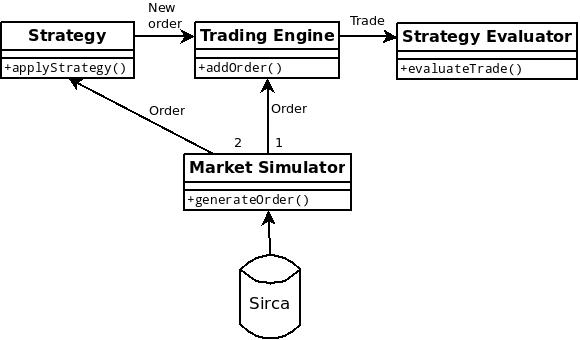
\includegraphics[width=0.8\textwidth]{architecture}
\caption{ATS Architecture Flowchart}
\label{fig:architecture}
\end{figure}

\section{Environment}
% Describe your testing environment: e.g. environment and/or tools used,
% limitations (e.g. things that are not tested)

% Software used during testing (if any)

\section{Data}
% Overview of test data (test cases).

% Test input files (order files)
% Result files (if any)

\section{Process}
% Illustrate your testing process i.e. how your team conducts testing using
% the test data described earlier (e.g. in which order). How do you make sure
% you do not break old features when introducing new features?

% Test configuration files


\end{document}
